\PassOptionsToPackage{bookmarks=false}{hyperref}
%% The first command in your LaTeX source must be the \documentclass command.
%\documentclass[sigconf]{acmart}
\documentclass[sigconf]{acmart}
\usepackage{xspace}
\usepackage{hyperref}
\usepackage{listings}
% \usepackage[ruled,vlined]{algorithm2e}
\usepackage{overpic}
\usepackage{amsmath}
\usepackage{alg}
\usepackage{subcaption}

\lstset{language=Java, showspaces=false, showtabs=false, breaklines=true,
  numbers=left, numbersep=1pt, numberstyle=\tiny\color{black},
  showstringspaces=false, breakatwhitespace=true, commentstyle=\color{pgreen},
  keywordstyle=\color{pblue}, stringstyle=\color{pred},
  basicstyle=\small\ttfamily, moredelim=[il][\textcolor{pgrey}]{$$},
  moredelim=[is][\textcolor{pgrey}]{\%\%}{\%\%}}

\newcommand{\name}{NAME\xspace}
\newcommand{\fixme}[1]{{\color{red}{\textbf{FIXME:#1}}}}

\AtBeginDocument{%
  \providecommand\BibTeX{{%
    \normalfont B\kern-0.5em{\scshape i\kern-0.25em b}\kern-0.8em\TeX}}}

\begin{document}

\title{Critical Survey 2: Relational Parametricity}

\author{Juyeon Yoon}
\affiliation{%
  \institution{School of Computing, KAIST}
  \city{Daejon}
  \country{Republic of Korea}
}
\email{juyeon.yoon@kaist.ac.kr}


\begin{abstract}
  So this critical survey needs abstract?

\end{abstract}

\maketitle

\section{Introduction}
\label{sec:intro}

Smartphones have become ubiquitous, and mobile platforms such as iOS and Android
have more users than any other computing plattorms. In particular, Android has
been very successful, occupying more than 80\% of the world-wide smartphone
market~\cite{idc-smartphones}. However, existing research show that many
software that run on the Android platform (i.e., apps) may not have been as
thoroughly tested as their desktop counterparts. A recent survey of Android
projects and developers shows that only 14\% of the studied open source
Android apps have any test cases at all, and less than 10\% have test cases
that achieve more than 40\% code coverage~\cite{Kochhar2015lp}. Considering
that most apps face high competition for the time and attention of users\footnote{It is reported that about 25\% of all installed apps are used only
  once by the user: \url{https://www.statista.com/statistics/271628/percentage-of-apps-used-once-in-the-us/}.}, error-prone apps
are at a significant disadvantage at retaining the user by providing positive
user experience.

One challenge reported in the survey is that automated testing has not been
widely adopted in the open source Android development community~\cite{Kochhar2015lp}. While other factors such as device fragmentation do indeed
contribute to the slow adoption of automated testing techniques for Android~\cite{Muccini2012pv}, one technical issue that hinders wider use of automated
testing for Android is the inherent fragility of GUI test cases. A relatively
small change in the appearance of an app can break test cases that traverse
the GUI~\cite{Coppola2016rd}.

This paper proposes a machine learning based test case repair technique for a
specific cause of test fragility, which is view identification failure~\cite{Coppola2019fv}. Typically, automated GUI testing framework for Android first
identifies a GUI element (i.e., a \emph{view}), such as a button, and
subsequently initiates a GUI event to emulate user interaction. For example,
the following is an example code snippet written using an automated GUI
testing framework called Espresso~\cite{}: it finds a button with view
identifier \lstinline+btnConfirm+ and clicks it.

\begin{lstlisting}
onView(withId(R.id.btnConfirm))
  .perform(click());
\end{lstlisting}

A view identification failure occurs when the latest modification to the app
source code changes the view identifier \lstinline+btnConfirm+ to
\lstinline+btnOk+, but the test case continues to find the same button using
the previous identifier. Consequently, the test execution terminates with an
\texttt{ViewMatchingException}, despite the fact that the logic of both the app and the
test case has not changed. The view identification failure is listed as one of
the major causes of Android test fragility in a recent survey of
Android test practices~\cite{Coppola2019fv}.
% \fixme{mention compile error?}\
The common cause of view identification failure is the fact that external
appearance of the app (i.e., the GUI design) can evolve even when the internal
logic of the app does not. This separation of concern, unfortunately, also
allows the mismatches between the app and the test code. However, it also
provides a ground for automated repair: if the underlying app logic has not
changed at all, or changed only slightly, we can expect that the new identifiers or
names given to the updated GUI element will be similar to the previous names.
If, for example, the latest GUI modification was simply to fix typos in view
identifiers, the old and the new ids will be lexically similar. Even if the
change was more than simple typo fix, as long as the core logic wrapped inside
the GUI remains largely the same, we expect the old and the new identifiers to
be semantically similar.

This paper presents an automated repair technique for view identification
failures based on both lexical and semantic similarities between view
identifiers. We formulate the repair problem as a classification problem:
given a pre-change identifier (used by the broken test case) and a set of
post-change ids (collected in the modified app source code), we classify
whether each of the post-change identifiers is potentially the one that
matches the pre-change identifier. Our classification model uses a set of
similarity features: lexical similarity (measured between two identifiers),
semantic similarity (measured between two sets of tokens taken from two
identifiers), and source code similarity (measured between code snippets
related to two identifiers). The results of classification is presented as a
ranking of post-change identifiers. An empirical evaluation based on real world view identification failures shows that the proposed approach can repair 72\% of the failures within 3 trials and precisely matched post-change identifiers for 48\% of the studied failures by ranking the correct one on top.

The remainder of the paper is organised as follows. Section~\ref{sec:repairing_vif} describes the view identification failure in more detail and introduces the formulation of our repair technique. Section~\ref{sec:experimental_setup} presents the experimental setup of the empirical evaluation, the results of which is reported in Section~\ref{sec:results}. Section~\ref{sec:threats} presents the threats to validity. Section~\ref{sec:related_work} introduces the related work, and Section~\ref{sec:conclusion} concludes.

\section{Repairing VIF By Identifier Matching}
\label{sec:repairing_vif}

This section describes what View Identification Failure (VIF) is and presents
our formulation of VIF repair as a classification problem.

\subsection{View Identification Failure}
\label{sec:vif}

The View class is the base class for all Android GUI widgets. An automated GUI
test case emulates user interaction by 1) identifying a specific view (such as
a button), and 2) invoking a specific GUI event (such as click). For the first
step, the test case typically uses unique properties of the view, such as the
given view identifier. View Identification Failure (VIF) occurs when an
automated GUI test case fails to specify a view to which it wants to invoke a
GUI event. This inconsistency is often caused by the fact that the GUI, i.e.,
the external appearance of an Android app, may go through modifications that
do not involve any change of the underlying logic of the app. If only the GUI
part of the app is changed, and not the test case code, then VIF occurs.

This paper specifically focuses on VIFs that involve outdated View
identifiers. All GUI widgets can be given identifiers in the layout resource files in XML format
that defines the visual structure in an Android application: these identifiers are accessible from within
the app source code via the automatically generated class named \lstinline+R.java+\ with \lstinline+R.id.+\ object. Views can be targeted by test cases via their identifiers.

Let us use the terms pre- and post-change identifier to refer to the outdated
identifier in the test code, and the new, modified identifier in the app code;
we will hereafter also use id to stand for view identifiers for the sake of
brevity. If the relationship between pre- and post-change ids are completely
arbitrary, an automated repair would not be feasible. As an artificial extreme
case, consider a random mapping between view ids of two different apps:
figuring out the arbitrary mapping would be clearly impossible.

Luckily, we expect most changes that result in VIFs to be still incremental,
i.e., that the functionalities of the app will largely remain the same. Either
the GUI change is completely superficial in the sense that it only changes the
GUI aspect of the app and not the underlying functionality, or the
functionality is also affected but not fundamentally. The continuity in the
functionality allows us a few different hypothesis, which we will consider in
the following sections.

\subsection{VIF Repair as a Classification Problem}
\label{sec:classification}

We formulate VIF repair as a classification problem. Let $A$ and $A'$ denote the App Under Test (AUT): $A$ is the original version before the GUI change, whereas $A'$ is the latest version after the GUI change. Let $T$ be the GUI test case before the GUI change that is now broken due to VIF. The pre-change view id, $i$, only appears in $T$. Finally, let $I_c$ be the set of all candidate post-change view ids that appear in $A'$:

\[I_c = \{i_c | i_c \in A'\}\]

VIF repair is essentially the problem of finding $i' \in A'$ such that $i'$ is
the modified version of $i$. Given a pair of pre- and post-change view ids,
$(i, i_c)$, we label the pair 1 if the pair is the correct match between the
same GUI widget with modified view ids, and 0 otherwise. If we can train a
classifier, $C$, of view id pairs based on this labelling, we can repair the
test $T$ that is broken by VIF as follows:

\[i' = i_c \mbox{ such that } i_c \in A' \wedge C(i, i_c) = 1\]
\[T' = T[i \leftarrow i_c]\]

We train a binary classifier $C$ for view identifier pairs, using actual view
identifier changes collected from open source Android app repositories. The
classification result is used to form a rank of potential match candidates,
$i_c$. Ideally, the correct match, $i'$, should be ranked at the top, and will
be used to update $T$ to $T'$ by replacing $i$ with $i'$.

\subsection{Similarity-based Input Features}
\label{sec:features}

We now turn our attention to the input features for the classification model.
Intuitively, we assume that pre- and post-change view ids will be still
similar to each other, due to the continuity in the underlying functionality
of the AUT.

\subsubsection{Lexical Similarity Feature}
\label{sec:lexical}

One common type of superficial GUI changes related to VIF is the systematic
change of view id naming convention. For example, it is possible that
the pre-change id did not include the GUI widget type (e.g., \lstinline+Confirm+), and the post-change id was modified so that it follows a naming convention
that requires the widget type is explicitly reflected in the id (e.g.,
\lstinline+buttonConfirm+ or \lstinline+btnConfirm+). With naming convention
changes, it is likely that part of the pre-change id remains the same in the
post-change id. Consequently, we expect the lexical similarity, captured
by Levenshtein distance~\cite{Levenshtein:1966sf}, to capture this
relationship. Levenshtein distance is a specific type of edit distance between
two strings, $a$, and $b$, which is formally defined as follows:

\begin{equation}
  lev(a, b) = \left\{\begin{array}{ll}
    |a|                                             & \mbox{if } |b| = 0      \\
    |b|                                             & \mbox{if } |a| = 0      \\
    lev(a[1:], b[1:])                               & \mbox{if } a[0] == b[0] \\
    1 + \min\left\{\begin{array}{l}lev(a[1:], b)\\lev(a, b[1:])\\lev(a[1:], b[1:]))\end{array}\right. & \mbox{otherwise}        \\
  \end{array}\right.
  \label{eq:lev}
\end{equation}

We hypothesise that the correctly matched pair, $(i, i')$, will have higher
lexical similarity than other pairs, for view modifications such as typo fixes
or application of new naming conventions.

\subsubsection{Semantic Similarity Feature}
\label{sec:semantic}

It is also possible that the the change resulted in VIF is more semantic than
the simple lexical addition or pre- or suffixes. If the change made to the
view id reflects the minor change in the underlying functionality, the
post-change view id may be still semantically similar to the pre-change id.
For example, \lstinline+btnConfirm+ may have been modified into \lstinline+btnOK+. Lexical similarity cannot detect such relationships, so we introduce
word embedding~\cite{Mikolov:2013rw} to measure semantic distance between two
view ids.

Since we want to exploit the semantic continuity in the functionality of the
app (reflected in the view identifiers), we use the embedding model that is
pre-trained for natural language corpus in English. However, the view
identifiers are not single words: they are rather composite words made up of
multiple tokens (such as `btn' and `Confirm'). To cater for the composite word
ids, we tokenise each identifier and apply the word embedding to the
constituent tokens. More formally, given two view ids, $i_1$ and $i_2$, and a pre-trained word2vec embedding model, $w2v$, the semantic similarity $sem(i_1, i_2)$ is computed as follows:

\[\tau_1 = \{t : \mbox{ token } t \mbox{ is part of } i_1\}, \tau_2 = \{t : \mbox{ token } t \mbox{ is part of } i_2\}\]
\[sem(i_1, i_2) = \min_{(t_i, t_j) \in \tau_1\times\tau_2}{cosine\_sim(w2v(t_i), w2v(t_j))}\]

We hypothesize that, for a superficial view id change from $i$ to $i'$ that
does not involve any significant change of the underlying app functionality,
$i$ and $i'$ are likely to be semantically similar to each other, reflecting
the continuity in app functionality. Given such similarity, it is also likely
that tokens $t$ and $t'$ from $i$ and $i'$ respectively have high cosine
similarity when embedded in vector forms. Note that when the changes made to
the given pre-change view id is simply addition of prefix or suffix, semantic
similarity will produce the highest similarity, because both pre- and
post-chagne view ids will include identical tokens.

\subsubsection{Code Similarity Feature}
\label{sec:codesim}

Given the degree of freedom in natural language, we cannot guarantee that
the use of lexical and semantic similarity is sufficient to capture all
relationships between pre- and post-change view ids. For example, suppose the
post-change view id is entirely consists of acronyms not contained in the word
embedding dictionary, or even non-English words: semantic similarity computed
via word embedding cannot cope with such changes. For such changes, we measure
the similarity between app source code elements that are connected to pre- and
post-change view ids.

Ideally, the source code element that best reflects the identity of the GUI
view under consideration would be its event listener, i.e., the method that
defines the behaviour of the view against incoming GUI events. However, there
are two challenges in identifying the event listener attached to a specific
view id. First, due to the way event listeners are attached to a GUI view, the
complete traceability between event listener code and a view id requires
dynamic analysis, which is not feasible due to the VIF in our context (i.e.,
we cannot execute the broken GUI test case). Second, not all view ids will
have attached event listener methods.

We tackle the first issue by developing a heuristic based on lightweight
static analysis. Using the static Java Parser, all of the method call expressions of the name with a postfix \texttt{Listener} are instrumented. The argument of the method should be the event handler attached to the object variable from which the method call is invoked. If the target object variable is assigned or declared by the previous method call containing \texttt{FindViewbyId}, \texttt{FindFragmentById}, or \texttt{FindById}, the first argument is extracted. Although this heuristic only captures the cases of using an anonymous function as a handler, we observed that this assumption covers most of the occurences of event handler registration on GUI components in the real-world Android applications. We avoid the second issue by considering any method that
explicitly refers to the given view id as relevant: let us call these methods
referrer methods. Compared to event listener, referrer methods will be less
specific to the view id, as the method may refer to multiple view ids.
However, we still expect that considering similarity between referrer methods
can help matching pre- and post-change view ids when the identifiers
themselves do not provide sufficient information.

To measure similarity between two arbitrary Android methods, we use the
\texttt{code2seq} embedding model that can produce vector embeddings of given
Java code~\cite{Alon2019ty}. Internally, \texttt{code2seq} represents code as
a collection of AST paths, which is any path that begins and ends at AST
terminal nodes. By considering multiple AST paths, \texttt{code2seq} learns to
embed the internal structure of the given AST. Given two view ids $i_1$ and $i_2$, and the $trace$ function that maps a view id to either event listener or referrer methods, the code similarity $csim(i_1, i_2$ is computed as follows:

\[m_1 = trace(i_1), m_2 = trace(i_2)\]
\[csim(i_1, i_2) = cosine\_sim(c2s(m_1), c2s(m_2))\]

We hypothesise that any modifications to the appearance of the app may not
involve code changes: consequently, we expect the code element that is traced
from the view ids will remain identical or highly similar between the
pre- and post-change view ids.

\subsection{Cascaded Classification}
\label{sec:cascade}

Our classification model uses the four similarity based input features
described in the previous section: lexical similarity, semantic similarity,
event listener method similarity, and referrer method similarity. However,
while the lexical and semantic similarity can be measured between any two view
ids, the two method similarity features may not be available. Consequently,
our technique contains multiple classifiers, each using a different number of
input features, and attempts to apply the one with the largest and the most
specific set of input features first. Given a classification algorithm $A$, we use the following classifiers:

\begin{itemize}
  \item $A(2)$: algorithm $A$ uses the lexical and semantic similarity as features.
  \item $A(3)$: algorithm $A$ uses lexical, semantic, and referrer method similarity as features.
  \item $A(4)$: algorithm $A$ uses all four similarity values as features.
\end{itemize}

Suppose we choose Random Forest (RF) as our classification algorithm. Given a
pair of view ids, the cascaded classification model will first check whether
both ids can be traced to event listener methods and referring methods: if so,
$RF(4)$ will be to classify whether the pair of ids points to the same GUI
widget or not. If listener similarity is not available, it will apply $RF(3)$.
Finally, if neither method similarity feature is available for both ids, then $
  RF(2)$ will be used with lexical and semantic similarity features.

\subsection{Test Case Repair}
\label{sec:repair}

We evaluate our GUI test case repair technique by simulating a VIF in a 
real-world Android application, \texttt{JustBe-Android} (\url{repo-address}), 
and subsequently applying our cascaded classification. For the sake of 
simplicity, we make the single FIF assumption, i.e., that there only exists a 
single VIF without any other test failures. Hence, it becomes possible to 
decide whether the simulated VIF has been successfully repaired simply by 
checking whether the test case broken by VIF passes after replacing the 
outdated pre-change view id with the matched post-change view id. The repair 
steps are described below:

\begin{enumerate}
\item \textbf{Localization of VIF:} Using the failure message either caused by 
a compiler error or a runtime \texttt{ViewMatchingException}, we localise the 
exact source code location of the outdated view identifier.

\item \textbf{Identification of referrer or event listener methods:} We try 
to identify whether a referrer or an event listener method exists for the 
pre-change view id. However, the AUT has already been changed and may no 
longer contain the pre-change view id. Consequently, we rewind the 
repository timeline by up to 10 commits, and search for the latest version 
in which the pre-change view id appeared in the AUT source code. If we find 
such a version, we apply the heuristic described in Section~\ref{sec:codesim}
to extract the method body. Afterwards, we construct the candidate view id 
pool in the post-change version (see Section~\ref{sec:subjects} for more 
details about how we construct the candidate view id pool).
  
\item \textbf{Ranking candidate identifiers by model:} According to the 
possible number of features identified from the previous step, the features 
are dynamically measured and fed into the cascaded classification model. 

\item \textbf{Iterative repair:} Once the list of the ranked candidates view 
ids is generated, our repair technique iteratively replaces the 
outdated view identifier with the candidate id in order, and terminates when 
the test case passes. In the presence of multiple outdated identifiers in the 
target test case, we check whether the failure message is changed each time 
the test case is re-executed with the new candidate id. We heuristically 
consider that the previous repair attempt was successful if another \texttt{
ViewMathcingException} from the new location is identified.
\end{enumerate}


\section{Experimental Setup}
\label{sec:experimental_setup}

This section describes the details of our experimental setup for the empirical
evaluation.

\subsection{Research Questions}
\label{sec:rqs}

We aim to answer the following research questions to evaluate our proposed approach.\\

\noindent\textbf{RQ1. Similarity Effectiveness:} How effective are the
individual similarity metrics described in Section~\ref{sec:features}? We
answer RQ1 by sorting all post-change candidate view ids according to each
individual similarity feature, and checking the rank of the correct
post-change candidate. We use $acc@n$ as the evaluation metric, which is the
number of pre-change view ids for which our technique can rank the correct
post-change counterpart within the rank of $n$. Ties are broken using max tie-breaking.\\

\noindent\textbf{RQ2. Model Effectiveness:} How effective is the cascade
classification model when compared to individual similarity features? We
evaluate multiple classification models including Logistic Regression (LR),
Support Vector Machine (SVM), Random Forest (RF), and Multi-Layer Perceptron
(MLP) in the context of cascade classification, and compare the results to
those of single similarity features. We compare different models using $acc@n$
evaluation metric too.

\begin{table}[ht]
  \caption{List of subject Android apps\label{tab:subjects}}
  \scalebox{0.8}{
    \begin{tabular}{lrrrr}
      \toprule
      Name                                       & \# of Commits & Textual & Referring & Listener \\ 
      \midrule
      akvo-caddisfly                             & 51            & 144     & 88        & 5        \\ 
      alltrack                                   & 1             & 2       & 2         & 1        \\ 
      andFHEM                                    & 22            & 47      & 13        & 1        \\ 
      android                                    & 156           & 148     & 53        & 6        \\ 
      android\_Skeleton                          & 11            & 23      & 16        & 0        \\ 
      android-money-manager-ex                   & 33            & 37      & 18        & 4        \\ 
      cominghome                                 & 2             & 2       & 1         & 1        \\ 
      poly-picker                                & 2             & 15      & 10        & 2        \\ 
      ts-android                                 & 78            & 75      & 39        & 2        \\ 
      Pr0                                        & 20            & 20      & 0         & 0        \\ 
      \midrule
      Total                                      & 376         & 513     & 240       & 22       \\ 
      \bottomrule
    \end{tabular}}
\end{table}

\subsection{Subjects}
\label{sec:subjects}

Table~\ref{tab:subjects} contains 10 Android apps that we study. All of these
apps use the Espresso test automation framework, and have been studied by
Coppola et al.~\cite{Coppola2019fv} for Android test fragility. From the
repositories of these 10 apps, we extract 376 commits that modify only
view ids and not the app code, as these commits are likely to result in VIF.
Each of the 376 commits provides 513 pairs of pre- and post-change view
ids, $(i, i')$. 

While all such pairs can provide the textual (i.e., lexical and semantic) 
similarity between two view ids, not all pairs yield referring methods or 
attached event listener methods. Table~\ref{tab:subjects} also shows how many 
pairs provide each of the similarity features described in 
Section~\ref{sec:features}. 

To evaluate our classification approach, we also need to define the pool of 
post-change candidate view ids. If the pre-change view id yields either a 
referring method, or an event handler method, we take all post-change view ids 
that yield the same type of method and consider them as the candidate 
post-change view id pool. However, if the pre-change view id is traced to 
neither a referring nor an event listener method, we take all post-change view 
ids that appear in the GUI layout resource of the ATU and consider all of them 
as the candidate post-change view id pool.

We apply 10-fold cross validation for evaluation of all models. The reported 
model performance is aggregated across the results from each fold: the result 
for each pair of $(i, i')$ is taken from the run in which the fold that 
contained the given pair was used for validation.

\subsection{Metrics, Models \& Environments}
\label{sec:models}

We measure the lexical similarity (i.e., Levenshtein distance), using
\texttt{nltk} library\cite{Bird2009hs}. To measure semantic similarity, we use \texttt{spiral}\cite{Hucka2018} to tokenise view
ids and the pre-trained word2vec embedding model\footnote{\url{https://drive.google.com/file/d/0B7XkCwpI5KDYNlNUTTlSS21pQmM/edit}} to measure semantic
distances between tokens. As explained in Section~\ref{sec:features}, the
similarity between two view ids is the maximum similarity between tokens from
each view id.

All the classification models we use are from \texttt{scikit-learn} version 
0.23.2~\cite{Pedregosa2011fu}. All classification models have been used with 
their default settiong. We use Logistic Regression with \texttt{lbfgs} solver 
and L2 regularisation, and Random Forest with 100 estimators and gini purity. 
We use SVM classifier with Radial Base Function (RBF) to introduce 
nonlinearity. Finally, our MLP classifier uses 100 neurons in the hidden layer, and relu activation function~\cite{Nair2010ts}. 

The empirical evaluation was conducted on machines equipped with Intel Core i7 
and 32GB of RAM. We use the word2vec embedding model in the \texttt{gensim} 
library~\cite{Rehurek2010bs}, and the publicly available version of code2seq 
which is built using TensorFlow version 1.0. Both have been executed using 
NVidia Titan X and CUDA 11.



\section{Results}
\label{sec:results}

This section presents the results from our empirical evaluation and answers
the research questions.

\begin{table*}[ht]
  \caption{Accuracy@n numbers for individual similarity features and their
    percentage against total number of pre-change ids that yield the corresponding
    similarity feature values\label{tab:individual_ranking}}
  \begin{tabular}{lrrrr}
    \toprule
    Accuracy & Lexical Similarity & Semantic Similarity & Referrer Similarity & Listener Similarity \\ \midrule
    $acc@1$  & 146 (28.46\%)      & 230 (44.83\%)       & 67  (27.92\%)       & 10 (45.45\%)        \\
    $acc@3$  & 222 (43.27\%)      & 334 (65.11\%)       & 145 (60.42\%)       & 15 (68.18\%)        \\
    $acc@5$  & 248 (48.34\%)      & 367 (71.54\%)       & 185 (77.08\%)       & 17 (77.27\%)        \\
    $acc@10$ & 294 (57.31\%)      & 414 (80.70\%)       & 211 (87.92\%)       & 21 (95.45\%)        \\
    \midrule
    Total    & 513 (100\%)        & 513 (100\%)         & 240 (100\%)         & 22 (100\%)          \\
    \bottomrule
  \end{tabular}
\end{table*}

\begin{figure*}[ht]
  \centering
  \begin{subfigure}{0.4\textwidth}
    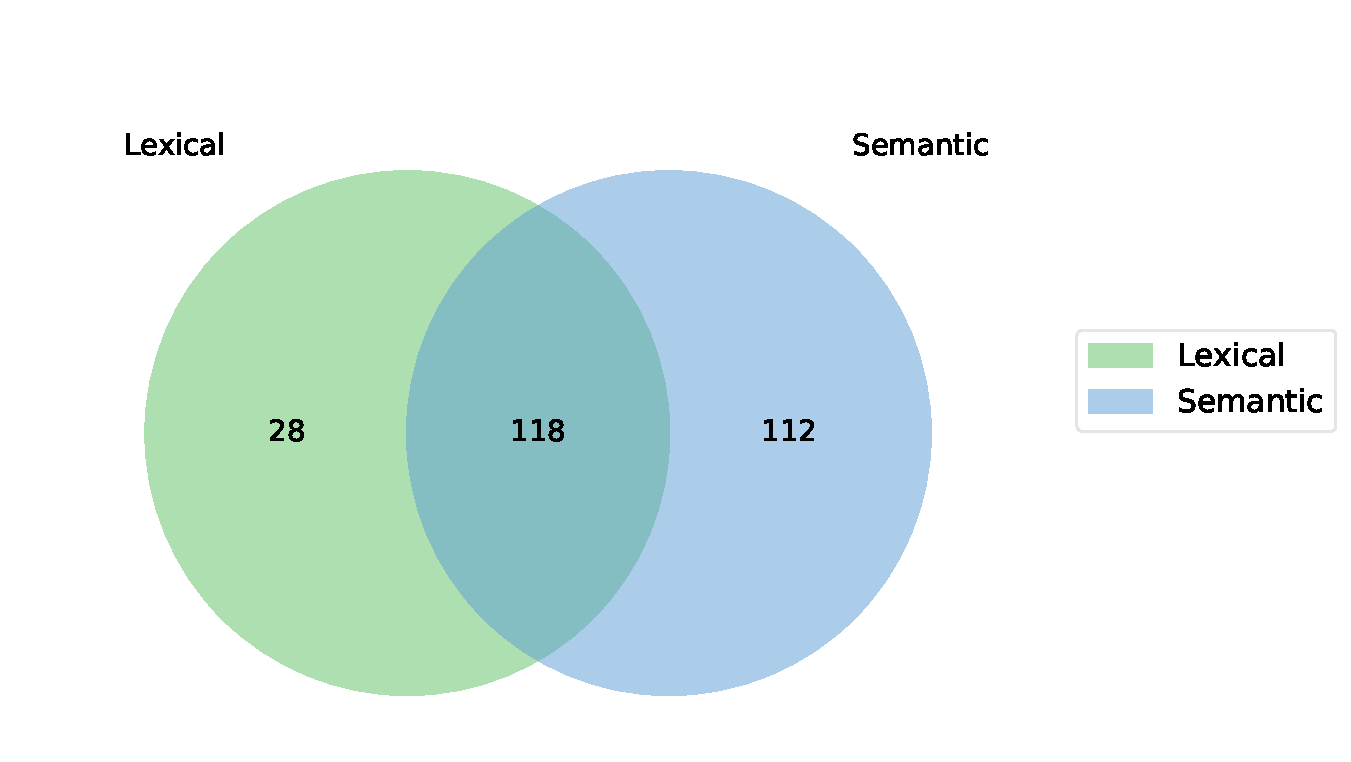
\includegraphics[width=70mm]{images/2_features_acc1.pdf}
    \caption{$acc@1$\label{fig:venn_2_1}}
  \end{subfigure}
  \hspace{1em}
  \begin{subfigure}{0.4\textwidth}
    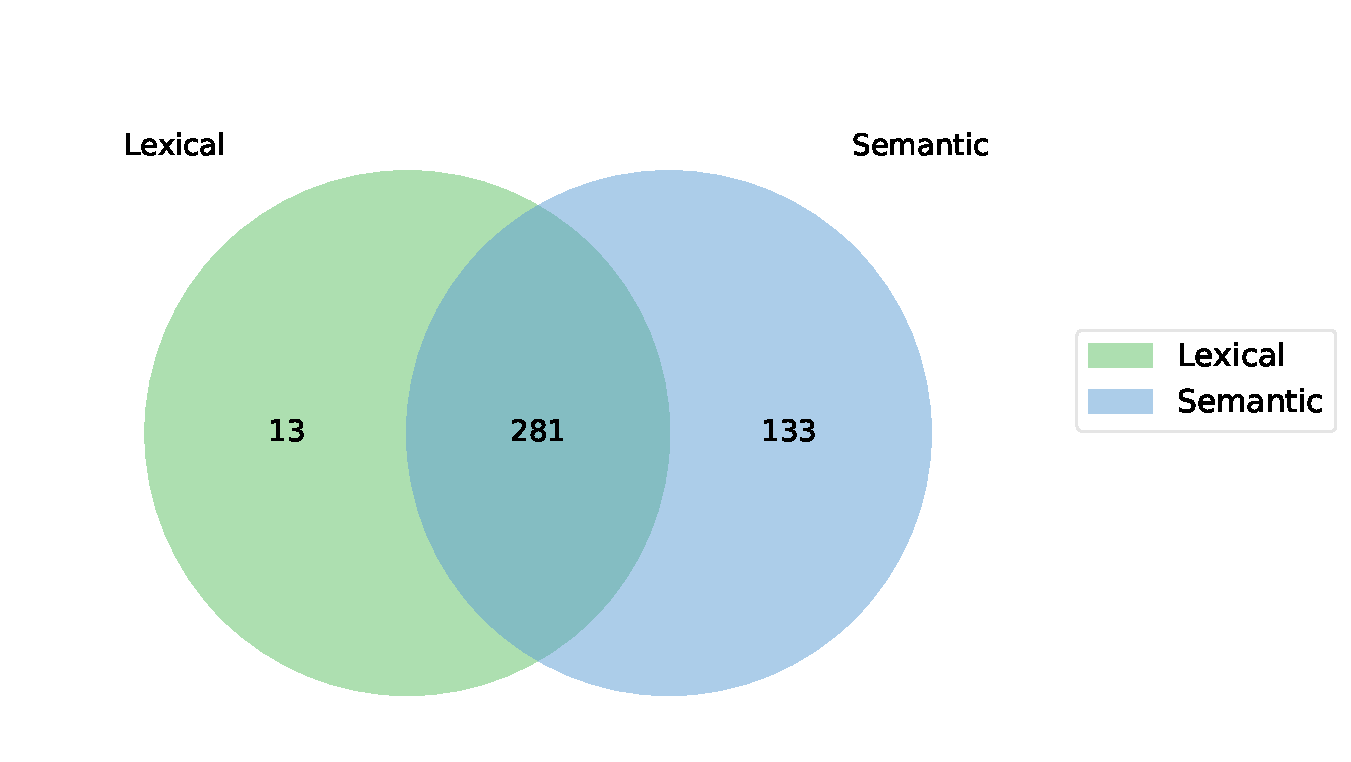
\includegraphics[width=70mm]{images/2_features_acc10.pdf}
    \caption{$acc@10$\label{fig:venn_2_10}}
  \end{subfigure}
  \Description{Venn diagram of $acc@1$ and $acc@10$ results produced by lexical and semantic similarity. Two features are complementary, each contributing unique results.}
  \caption{Venn diagram of $acc@1$ and $acc@10$ results produced by lexical and semantic similarity. Two features are complementary, each contributing unique results.\label{fig:venn_2}}
\end{figure*}

\begin{figure*}[ht]
  \centering
  \begin{subfigure}{0.4\textwidth}
    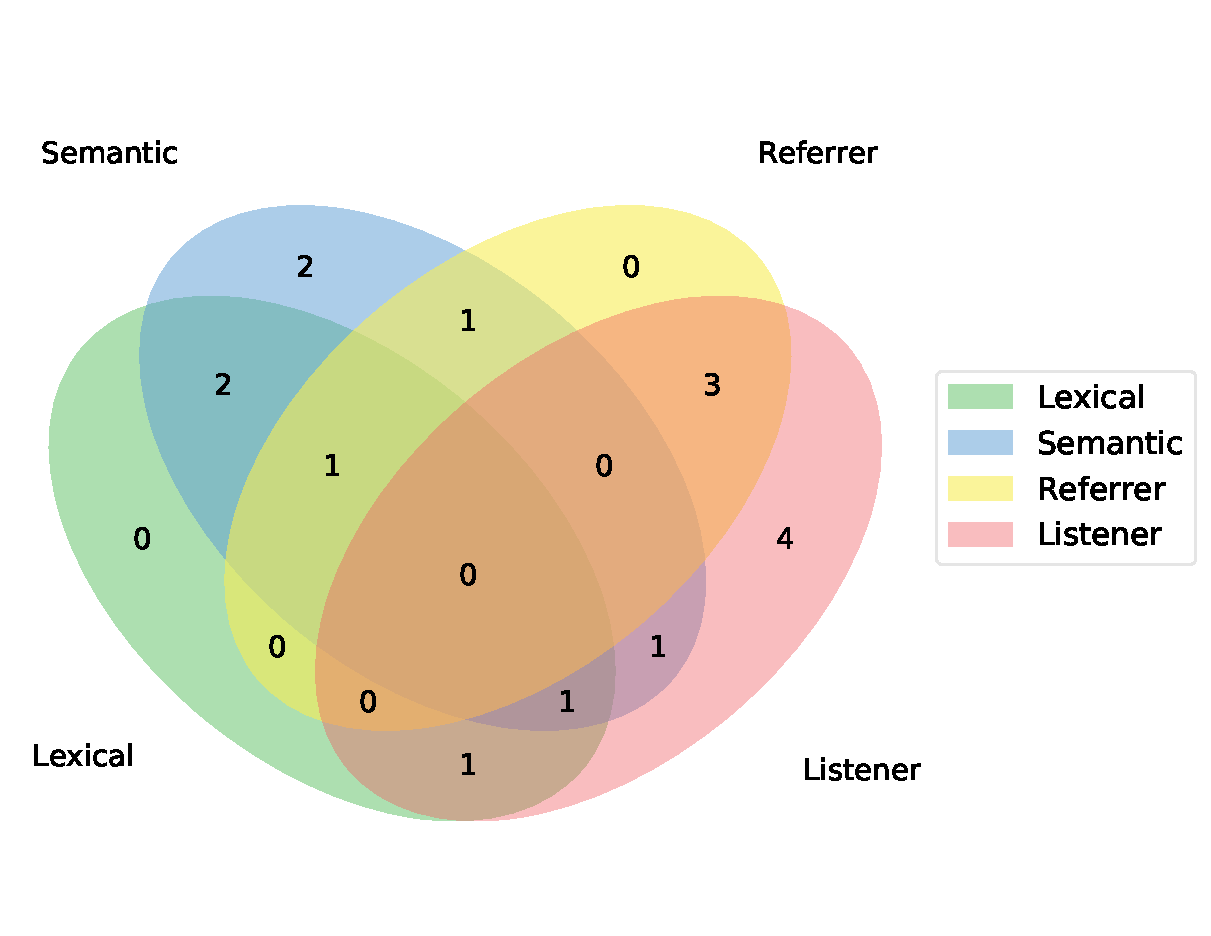
\includegraphics[width=\textwidth]{images/4_features_acc1.pdf}
    \caption{$acc@1$ (10 view ids)\label{fig:venn_4_1}}
  \end{subfigure}
  \hspace{1em}
  \begin{subfigure}{0.4\textwidth}
    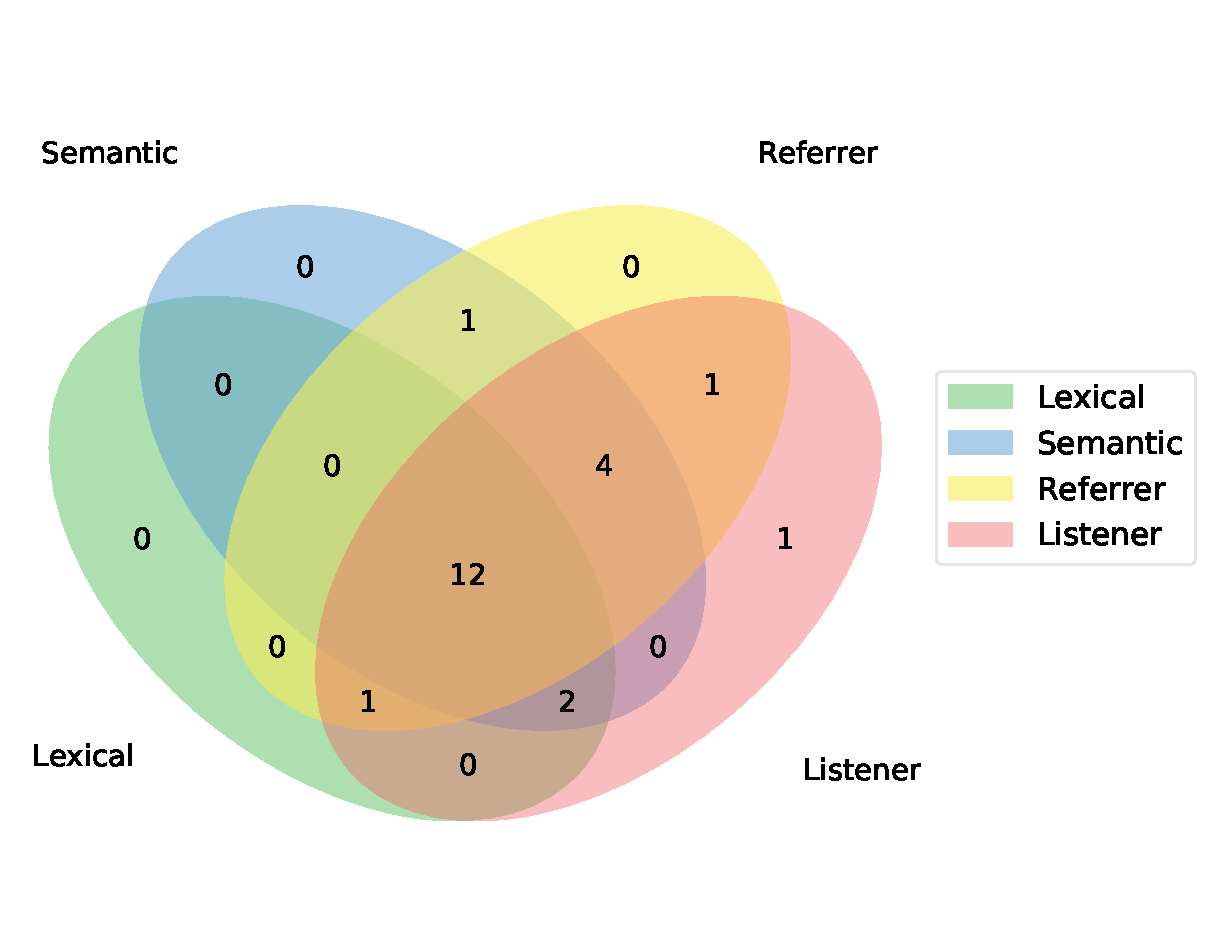
\includegraphics[width=\textwidth]{images/4_features_acc10.pdf}
    \caption{$acc@10$ (21 view ids)\label{fig:venn_4_10}}
  \end{subfigure}
  \Description{Venn diagram of $acc@1$ and $acc@10$ results produced by all four similarity features for 22 view ids: note that semantic and listener similarity features make unique contribution to $acc@1$.}
  \caption{Venn diagram of $acc@1$ and $acc@10$ results produced by all four similarity features for 22 view ids: note that semantic and listener similarity features make unique contribution to $acc@1$.\label{fig:venn_4}}
\end{figure*}

\begin{table*}[ht]
\caption{Accuarcy@n numbers for cascade classification models: (2) models use lexical and semantic similarities, (3) adds referrer similarity, and (4) adds listener similarity. Best results are typeset in \textbf{bold}.\label{tab:cascade}}
\scalebox{0.9}{
\begin{tabular}{l|rr|rrr|rrr|rrr|rrr}
\toprule
Accuracy & Lexical & Semantic & $LR(2)$ & $LR(3)$ & $LR(4)$ & $RF(2)$ & $RF(3)$ & $RF(4)$ & $SVM(2)$ & $SVM(3)$ & $SVM(4)$ & $MLP(2)$ & $MLP(3)$ & $MLP(4)$ \\ \midrule
$acc@1$  & 146     & 230      & 188   & 233   & 236   & 189   & 236   & 240   & 55     & 153    & 159    & 196    & \textbf{248}    & 248    \\
$acc@3$  & 222     & 334      & 326   & 366   & 367   & 286   & 329   & 333   & 90     & 189    & 197    & 329    & \textbf{371}    & 368    \\
$acc@5$  & 248     & 367      & 364   & 404   & \textbf{406}   & 321   & 371   & 372   & 105    & 207    & 214    & 367    & \textbf{406}    & 404    \\
$acc@10$ & 294     & 414      & 410   & 435   & \textbf{437}   & 336   & 396   & 396   & 133    & 219    & 227    & 408    & 433    & 432    \\
\bottomrule
\end{tabular}}
\end{table*}

\subsection{RQ1. Similarity Effectiveness}

Table~\ref{tab:individual_ranking} shows the $acc@n$ with $n \in \{1, 3, 5,
  10\}$ for all four individual similarity metrics. Note that the total number
of pre-change ids that yield these similarity values are different: we can
measure lexical and semantic similarity for all 513 studied pre-change view
ids, but referrer similarity for only 240 view ids, and listener similarity
for only 22. For fairer comparison between different similarity features, we
also report all $acc@n$ results as percentages against the total number of
relevant view ids (which is shown in the Total row).

Lexical and semantic similarity can be directly compared to each other as they
can be measured for all 513 studied view ids. Here, the semantic similarity
clearly shows better performance for all $n$ values. A closer analysis shows
that two similarity features are complementary. Figure~\ref{fig:venn_2}
contains Venn diagrams of $acc@1$ and $acc@10$ results produced by these two
similarity features. While there is a large intersection, each similarity
feature also makes unique view identifications.

While the small number of view ids with extractable event listener method
bodies means that more experimentation is needed before generalisation, the
listener similarity shows the highest highest $acc@1$ accuracy
percentage-wise. There are more view ids with referrer methods, but the
percent-wise $acc@n$ values are all lower than their counterparts produced by
listener similarity. We cautiously posit that listener similarity has more
specificity with respect to view ids than referrer similarity, which is
expected due to the fact that referrer methods are likely to make reference to
multiple view ids (e.g., setting up and attaching event listeners to multiple
widgets). This is also reflected in the Venn diagram of results from all four
similarity features shown in Figure~\ref{fig:venn_4}.


\subsection{RQ2. Model Effectiveness}

Table~\ref{tab:cascade} contains the results obtained from various cascade
classification models. We compare models that use two features (lexical and
semantic similarity), three features (plus referrer similarity), and four
features (plus listener similarity). Compared to two feature models, three
feature models show significantly improved accuracy, showing that the
inclusion of source code similarity helps identifying the correct post-change
view id. However, the small number of view ids for which the listener
similarity is available means that the improvement from three feature model to
four feature model is not significant.

Figure~\ref{fig:model_4} shows detailed break-down of $acc@1$ and $acc@10$
results produced by different cascaded models. The model that performs the
best is MLP, followed by RF and LR. However, while MLP overlaps significantly
with LR, we can observe that RF contributes the largest number of unique
$acc@1$ cases, which is 35. The same trend is observed in the Venn diagram for
$acc@10$. We suspect whether RF is more prone to overfitting to the data
compared to other classifiers.

\begin{figure}
  \centering
  \begin{subfigure}{0.45\textwidth}
    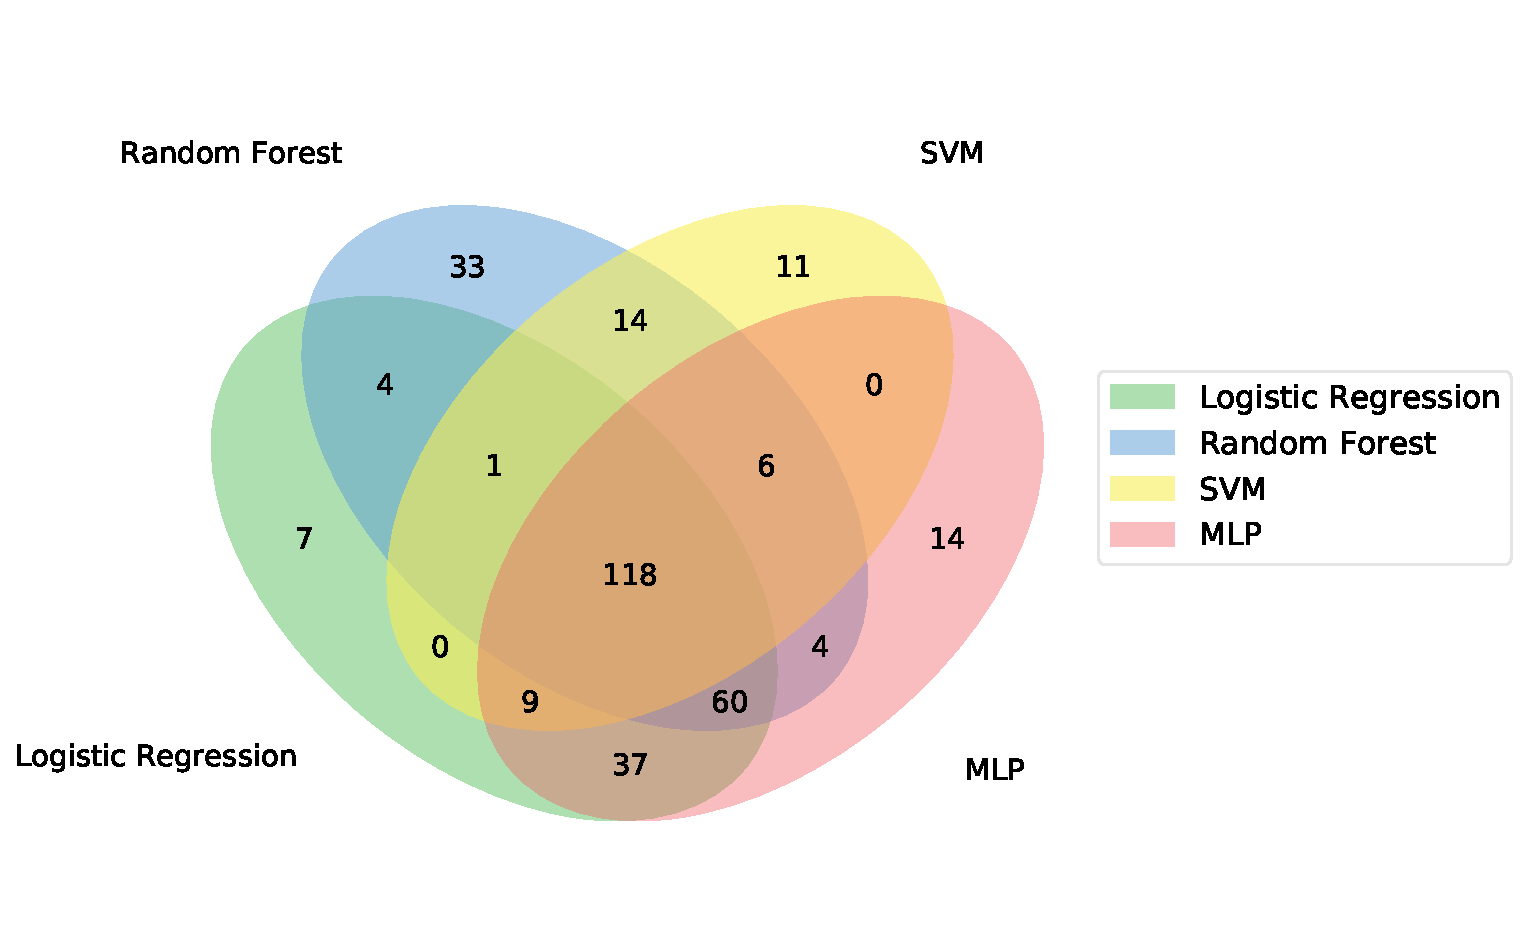
\includegraphics[width=70mm]{images/4_models_acc1.pdf}
    \caption{$acc@1$\label{fig:model_4_1}}
  \end{subfigure}
  \begin{subfigure}{0.45\textwidth}
    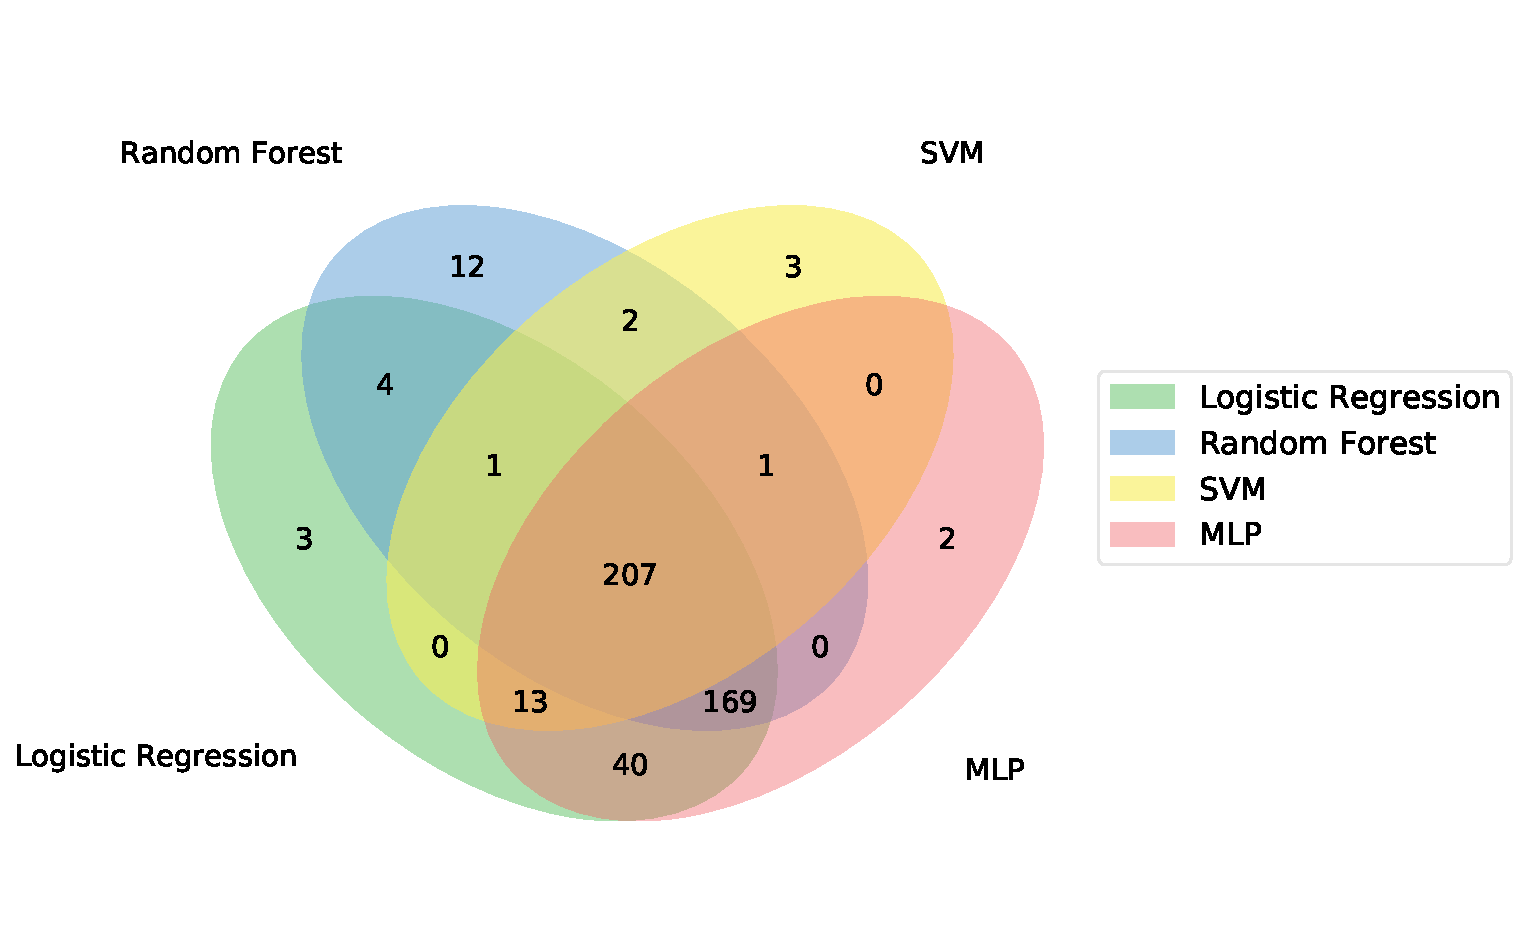
\includegraphics[width=70mm]{images/4_models_acc10.pdf}
    \caption{$acc@10$\label{fig:model_4_10}}
  \end{subfigure}
  \Description{Venn diagram of $acc@1$ and $acc@10$ results produced by cascaded classification models using four different classifiers.}
  \caption{Venn diagram of $acc@1$ and $acc@10$ results produced by cascaded classification models using four different classifiers.\label{fig:model_4}}
\end{figure}

\section{Threats to Validity}
\label{sec:threats}

The most serious threat to our study is the limited scope of studied apps. We 
only consider ten open source Android apps from those studied by Coppola et 
al.~\cite{Coppola2016rd}. First, the small sample size may mean that the 
results are biased. Second, it is possible that the degree of adoption of 
automated GUI testing in open source Android developer community is 
significantly different from that of closed source developers, in which case 
generalisation of our results may be difficult. While only further study can 
provide evidence for wider generalisation, closed source Android ecosystem may 
be difficult to study. We try to avoid threats to internal validity by 
choosing classification models implemented by a widely used open source 
framework that stood public scrutiny (scikit-learn~\cite{Pedregosa2011fu}).

\section{Related Work}
\label{sec:related_work}

While automated repair of program under test has been widely studied~\cite{Forrest:2009hi,Nguyen:2013aa,Mechtaev2016rw,Yuan2018zl,Wen2018dk}, automated
repair of test cases remain relatively unexplored. A closely related topic is
that of test augmentation, which aims to augment an existing test suite so
that it becomes adequate against an evolved program~\cite{Santelices2008aa,Xu:2011uq}. However, augmentation typically concerns making a test suite more
adequate by adding new test cases, whereas our approach aims at repairing
individual test cases by resolving VIFs.

VIF is part of GUI test case fragility~\cite{Coppola2016rd}: by fragility, we
mean that the test case can be easily broken by commits to the program under
test that are not bug inducing. It can be considered as a specific form of
test flakiness~\cite{Thorve2018vf,Bell2018fe}, which refers to
test cases whose outcome changes due to reasons unrelated to the correctness
of the program under test (e.g., unintended nondeterminism, or randomness in
environmental factors). However, fragility tends only to break test cases,
whereas flakiness in general means the test result oscillate between pass and
fail randomly. While there are studies that investigates the relationship
between code smells in test cases and flakiness~\cite{Palomba2017eq}, a direct
repair of test flakiness remains challenging.

\section{Conclusion}
\label{sec:conclusion}

We present a machine learning based resolution technique for View
Identification Failures (VIFs) to address test fragility in automated Android
GUI test cases. Based on the assumption that changes made to view ids are not
deeply coupled to changes in the functionality of the app, we hypothesise that
pre- and post-change view ids will be similar to each other, and evaluate
different similarity measures to match pre- and post-change view ids. We
formulate the problem as classification of pre- and post-change view id pairs,
and evaluate four different types of similarity features for their
classification effectiveness: lexical similarity, semantic similarity,
referrer method similarity, and event listener method similarity. The analysis
of individual similarity features show that different similarity features are
complementary to each other. Based on this, we introduce a cascaded
classification model that uses a set of different classification models that
use different sets of available features. Empirical evaluation of the cascaded
classification models shows that it can precisely match about 48\% of view id changes collected from real world open source Android apps, and can locate the correct post-change view identifier within top 3 candidates for 72\% of the cases.

\bibliographystyle{ACM-Reference-Format}
\bibliography{newref}

\end{document}

